\documentclass{article}

% Language setting
% Replace `english' with e.g. `spanish' to change the document language
\usepackage[french]{babel}

% Set page size and margins
% Replace `letterpaper' with`a4paper' for UK/EU standard size
\usepackage[letterpaper,top=2cm,bottom=2cm,left=3cm,right=3cm,marginparwidth=1.75cm]{geometry}

% Useful packages
\usepackage{amsmath}
\usepackage{graphicx}
\usepackage[colorlinks=true, allcolors=blue]{hyperref}
\usepackage{listings}
\usepackage{xcolor}

\definecolor{codegreen}{rgb}{0,0.6,0}
\definecolor{codegray}{rgb}{0.5,0.5,0.5}
\definecolor{codepurple}{rgb}{0.58,0,0.82}
\definecolor{backcolour}{rgb}{0.95,0.95,0.92}

\lstdefinestyle{mystyle}{
    backgroundcolor=\color{backcolour},   
    commentstyle=\color{codegreen},
    keywordstyle=\color{magenta},
    numberstyle=\tiny\color{codegray},
    stringstyle=\color{codepurple},
    basicstyle=\ttfamily\footnotesize,
    breakatwhitespace=false,         
    breaklines=true,                 
    captionpos=b,                    
    keepspaces=true,                 
    numbers=left,                    
    numbersep=5pt,                  
    showspaces=false,                
    showstringspaces=false,
    showtabs=false,                  
    tabsize=2
}

\lstset{style=mystyle}
\title{[MIF01]Rapport projet}
\author{KASMAMYTOV Eldar et BERTOLONE Melvyn}

\begin{document}
\maketitle

\begin{abstract}
Dans le cadre du premier semestre de M1 Informatique à l'Université Claude Bernard Lyon 1. Nous avons développé une application de gestion de CV dans l'unité d'enseignement MIF01.

\end{abstract}

\section{Introduction}
Nous devions développer une application de gestion de CV en respectant des contraintes fortes quant au choix des technologies de développement (Java) avec pour bibliothèque d'interface graphique \textit{JavaFX}, de qualité du code (utilisation d'un \textit{chekstyle} spécifique), d'intégration continue (Pipelines CI/CD), et de fonctionnalités à développer. Nous avons utilisé un dépôt git (forge de L'UCBL) afin de centraliser le code, faciliter le développement collaboratif de celui-ci, aider à l'intégration et à la gestion des différentes versions de l'application.
\subsection{Interface utilisateur et travail réalisé}
Il nous était demandé de réaliser une application en GUI (Figure \ref{fig:UI-CV-search}) ayant les fonctionnalités suivantes :
\begin{enumerate}
\item Différentes stratégies de sélection des candidats (Figure \ref{fig:UI-Search}) :
    \begin{enumerate}
        \item Toutes les compétences du candidat supérieur/inférieur ou égal à n\%
        \item Au moins une compétence du candidat supérieur/inférieur ou égale à n\%
        \item la moyenne des compétences du candidat supérieur/inférieur ou égale à n\%
    \end{enumerate}
\item Prise en compte de l'expérience professionnel.
\item Affichage des notes moyennes des candidats.
\item Affichage des années d'ancienneté des candidats.
\end{enumerate}
Nous devions aussi réaliser des fonctionnalités supplémentaires qui n'étaient pas précisées dans le "cahier des charges" du projet. Nous avons choisi d'implémenter les fonctionnalités supplémentaires suivantes : 
\begin{enumerate}
\item Autocomplétion pour l'écriture des labels de compétences. 
\item Fonctionnalité de tri pour la liste des candidats :
    \begin{enumerate}
            \item Par compétences (ordre croissant/décroissant).
            \item Par noms (ordre croissant/décroissant).
        \end{enumerate}
\item Modification de l'interface graphique.
\end{enumerate}
Nous détaillerons dans ce rapport (Section 2) les méthodes d'implémentations ainsi que le \textit{patron de conception} utilisé pour chaque fonctionnalité.

\begin{figure}[!tbp]
\centering
\begin{minipage}[b]{1\textwidth}
    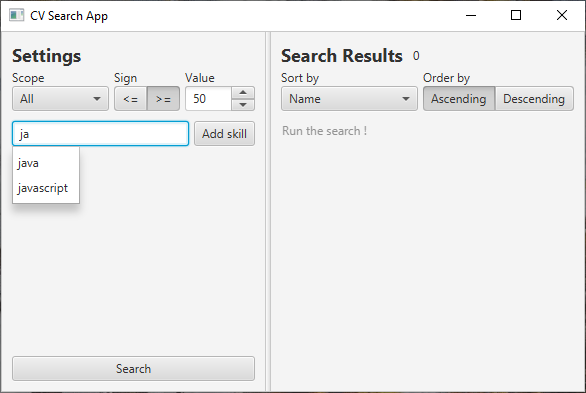
\includegraphics[width=\textwidth]{UI-CV-search.PNG}
    \caption{\label{fig:UI-CV-search}Interface utilisateur.}
    \end{minipage}
\begin{minipage}[b]{1\textwidth}
    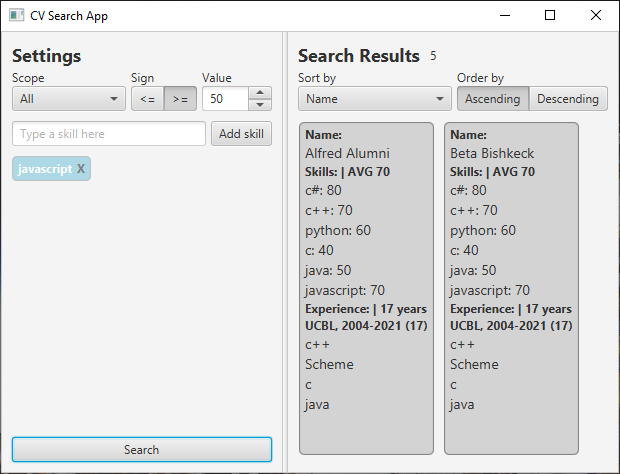
\includegraphics[width=\textwidth]{VC-searched.PNG}
    \caption{\label{fig:UI-Search}Interface utilisateur avec une recherche de compétence en JavaScript.}
    \end{minipage}
\end{figure}
\newpage
\section{Patron de conception}
En informatique, et plus particulièrement en développement logiciel, un \href{https://fr.wikipedia.org/wiki/Patron_de_conception}{Patron de conception} (souvent appelé \textit{design pattern}) est un arrangement caractéristique de modules, reconnu comme bonne pratique en réponse à un problème de conception d'un logiciel. Il décrit une solution standard, utilisable dans la conception de différents logiciels.
\subsection{Patron de conception \textbf{MVC}}
Nous avons fait le choix d'utiliser le patron de conception Modèle-Vue-Contrôleur (MVC) pour gérer la logique derrière les actions graphiques de l'utilisateur.

Contrairement à l'implémentation classique des vues dans ce patron de conception (où chaque fonctionnalité a sa propre vue et son propre modèle), nous avons fait le choix d'utiliser un seul fichier FXML servant de vue.

Afin d'initialiser l'interface graphique une chaine d'appels s'effectue jusqu'à l'appelle de la fonction \textbf{loadFxml()} (Figure \ref{fig:loadFXML_chain}).

Dans cette configuration, il faut spécifier dans le contrôleur (CvSearchController.java) les différents éléments graphiques nécessitant une gestion d'événements (par exemple, le fait d'appuyer sur un bouton). Cette spécification des élément se fait en utilisant une balise @FXML au-dessus de l'écriture des données membres dans le corps de notre contrôleur :
\begin{lstlisting}[language=java]
@FXML
private ToggleButton signSelectorGreater;
\end{lstlisting}


\begin{figure}[!tbp]
\centering
\begin{minipage}[b]{1\textwidth}
    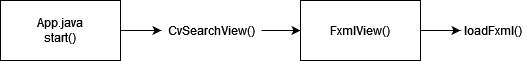
\includegraphics[width=\textwidth]{FXMLLoader.png}
    \caption{\label{fig:loadFXML_chain}Chaine d'initialisation pour le fichier FXML.}
\end{minipage}
\end{figure}



\subsection{Patron de conception Stratégie}
Nous avons fait le choix d'utiliser le patron de conception Stratégie pour l'implémentation de la fonctionnalité de recherche des CV, ce patron paraissait le plus adéquat étant donné que nous étions dans le cas où nous devions utiliser un algorithme spécifique, en fonction d'\textbf{une} entrée utilisateur pendant que l'application s'exécutait. \\
En effet, dans notre application, pour la sélection des stratégies de recherche, nous utilisons un bouton \textbf{scopeSelector}, quand l'utilisateur lance la recherche, l'événement est récupéré par le contrôleur qui décide "automatiquement" (Figure \ref{fig:SearchStrategyUML}) quelle fonction de recherche utiliser.
Nous utilisons aussi ce patron pour la sélection des méthodes de tri des CV (par nom ou compétences).

\begin{figure}[!tbp]
\centering
\begin{minipage}[b]{1\textwidth}
    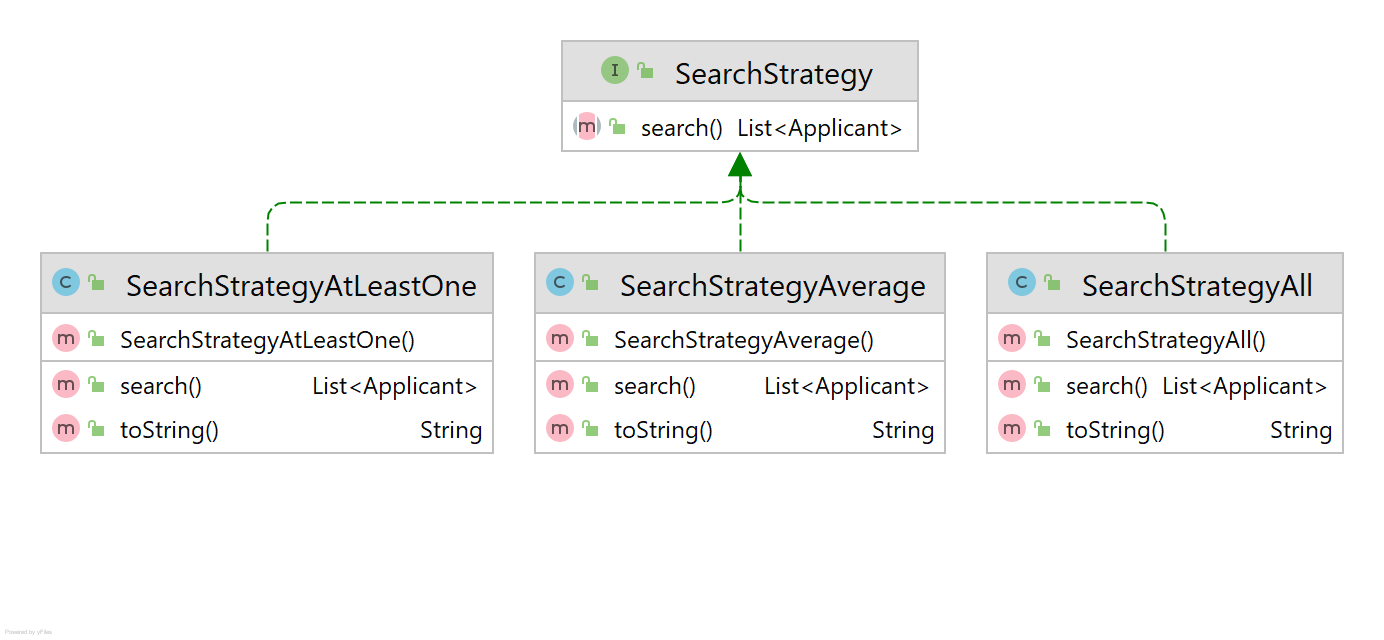
\includegraphics[width=\textwidth]{SearchStrategy.png}
    \caption{\label{fig:SearchStrategyUML}Diagramme UML pour le sélecteur de stratégies.}
\end{minipage}
\end{figure}


\subsection{Patron de conception Observer}
Nous avons fait le choix d'utiliser le patron de conception Observer pour l'autocomplétion des labels lorsque l'utilisateur renseignes les compétences qu'il veut pour sélectionner les CV.
\begin{lstlisting}[language=java]
addSkillField.setOnKeyTyped(event -> {
    Set<String> res = findMatchingSkills(addSkillField.getText());
    searchSuggestions.getItems().clear();
    res.forEach(this::addSearchSuggestion);
})
\end{lstlisting}
Nous l'avons implémenté de la façon suivante :\\
Un "observer" attend une entrée utilisateur dans la vue, quand l'utilisateur tape une lettre dans le champ de recherche, un parcours de la liste des compétences existante (dans le modèle des appliquant) sera effectué, si un mot "match" avec l'entrée utilisateur, cela mettra à jour la vue avec les mots suggérés (Cf. Code ci-dessus).

\subsection{Patron de conception Singleton}
Nous avons fait le choix d'utiliser le patron de conception Singleton pour l'implémentation de la classe "SearchState"(Figure \ref{fig:SearchState}).
Nous trouvions que l'implémentation de ce patron se prêtait bien à cette classe, étant donné que nous avions le besoin de restreindre l'instanciation de cette classe à une seule instance.\\
Nous avions besoin d'exactement un objet pour coordonner les actions à travers le système.

\begin{figure}[!tbp]
\centering
\begin{minipage}[b]{0.5\textwidth}
    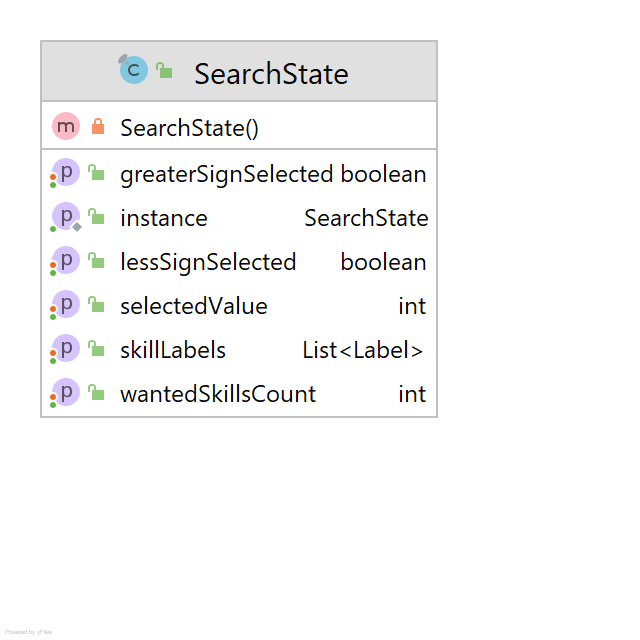
\includegraphics[width=\textwidth]{SearchState.png}
    \caption{\label{fig:SearchState}Diagramme UML pour la classe SearchState.}
\end{minipage}
\end{figure}
\newpage
\section{Éthique}
L'éthique dans le recrutement est un sujet vaste et complexe, avant d'analyser les questions éthique de nos choix de conceptions et de l'implémentation des fonctionnalités dans l'application, il nous semblait important de faire un rapide point sur les différents niveaux à distinguer dans le processus de recrutement, afin de poser les bases de notre analyse, et de replacer dans un contexte correct la question de l'éthique dans le développement informatique pour la sélection des futurs employés d'une entreprise.
\subsection{Les 4 niveaux à distinguer}
Dans le Guide du recrutement non discriminatoire\cite{ied_proc_recrutement}  de l'Institut Éthique & Diversité, quatre niveaux pour assurer un "bon" processus de recrutement et d'accueil dans l'entreprise :
\begin{enumerate}
    \item Risque judiciaire.
    \item Égalité de traitement.
    \item Égalité des chances.
    \item Gestion de la diversité.
\end{enumerate}
Attardons-nous sur l'égalité de traitement, elle est définie dans le guide comme la sélection objective des profils. Il est important de noter qu'une sélection objective n'est pas une discrimination, en effet une sélection n'est pas sociale et se doit de respecter le droit, ainsi que de sélectionner le meilleur profil pour le poste proposé.
\subsection{La sélection des profils dans notre application}
Comme demandé dans le "cahier des charges" du projet, nous avons implémenté différentes fonctionnalités pour la sélection des CV.

Si l'on se réfère encore au Guide du recrutement non discriminatoire\cite{ied_proc_recrutement}, nous ne faisons pas de traitement "discriminatoire" directement dans le code notre application pour la sélection des profils. En effet, c'est l'utilisateur qui est chargé de donner les indications au logiciel pour sélectionner les profils \textbf{seulement sur la base des compétences}. \\
Notre application effectue un traitement égalitaire dans la liste des CV en respectant les contraintes fournies par l'utilisateur.\\
Cependant l'un des problèmes éthiques que l'application peut soulever est la notation des profils par une valeur moyenne stricte, en effet, cela créer une force morale implicite pouvant pousser inconsciemment le recruteur à sélectionner les profils ayant une valeur moyenne de compétences élevé sans prendre en compte l'individu et son expérience professionnel antérieur.
\subsection{La responsabilité de l'utilisateur}
Dans un processus de recrutement non discriminatoire, la première étape à respecter est la définition d'une grille de sélection précise permettant de déterminer quelles seront les candidatures à écartées et quelles seront les candidatures qui seront présélectionnées.

\section{Tests}
Nous testions au fur et à mesure d'un point de vue utilisateur les limites de l'application. Par exemple qu'un enchainement d'actions prédéfinies sur l'interface nous retourne le résultat attendu, que la fenêtre soit bien responsive. Cette méthode nous a permis de couvrir une grande partie des problèmes que l'utilisateur final pouvait rencontrer par l'utilisation directe de l'application.
Nous avons aussi réalisé un ensemble de test manuel afin de jauger les limites de l'application en "profondeur", pour la gestion des données vides par exemple, test des données de mauvais type, etc.



\bibliographystyle{alpha}
\bibliography{sample}

\end{document}